\subsection{Use concepts and language that your user understands}

A essential point is that the user must be able to understand what we are trying to communicate. We must create a fluid, 
easy interaction between the user and the representation of the data. Therefore we must speak with the language of 
the ordinary person, using common vocabulary, avoiding specialist jargon and communicating in the simplest, 
clearest manner. The representation of information plays a fundamentally important role, enabling the user to absorb 
the underlying meaning in a natural way.\\

\subsubsection*{Suggested strategies} 

\begin{itemize}
    \item Consider what type of representational format is most appropriate to the task.
    
    \item Provide the resources needed to help the user to understand and place the information in context.

    \item Consider carefully which type of representation fits better to which kind of data. a graph may not necessarily be the clearest representation.

    \item If using graph is the best solution, consider carefully which type to use. For example, 
    if you are representing individual samples and want to show the density, lean towards a density graph; if presenting data discriminated by gender,
    maybe a pie chart is the most appropriate.
\end{itemize}

\subsubsection*{In the context of Aire Guru \ldots} 

The Aire Guru tool presents the information in the native language of the city (Spanish), avoids using difficult scientific terminology, instead using simple vocabulary and a 
straightforward style. Colors and graphic resources are used, as are icons. In addition, the site uses a unified design language to represent data,
giving the user a consistent visualization experience. \\

One of the objectives is to represent pollution by geographic area of the city, which is why a map has been used - the 
obvious and familiar visual image of the different places in the city. The pollution index shows an indicator with 
five levels represented by a color scale from turquoise to red - "Good" "Fair" "Poor" "Bad" and "Unhealthy". 
This color-coding is consistent with the colors which are used in official sources, thereby avoiding confusion for any 
user who might consult official sources.

\begin{figure}[ht]
    \centering
    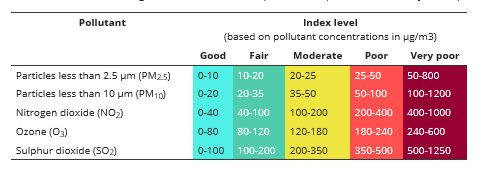
\includegraphics[width=12cm]{Figure_4_4_1_EAQI_Levels}
    \caption{EAQI Levels}
\end{figure}
\begin{center}
    \bf{        
    Figure 4.4.1. EAQI Levels}
\end{center}

These icons represented in the Figure 4.4.2 are used to help the user get an immediate idea of the pollution level, since they are even more
decriptive and self-explanatory than just colors alone. Danger is, of course, almost universally indicated by 
the colour red, and is therefore used appropriately. However, not all cultures have the same perception about
blue or green, missing what they indicate. In this case we have a limited geographic market, so it isn't an issue.\\

\begin{figure}[ht]
    \centering
    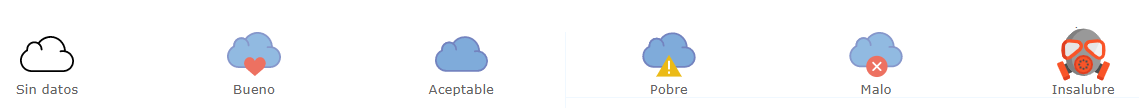
\includegraphics[width=10cm]{Figure_4_4_2_EAQI_Icons}
    \caption{Iconografica Aire Guru}
\end{figure}

\begin{center}
    \bf{        
    Figure 4.4.2. EAQI Icons}
\end{center}
For the graphs that show variations in time, we have chosen line graphs as being most appropriate,
since they are good at showing continuous evolution over a period of time. To represent the different components of the AQI, we use a
graph of stacked bars, since it is easy to see what proportion of the total AQI is formed by which pollutant. \\

\begin{figure}[ht]
    \centering
    \subfigure[AQI Evolution]
        {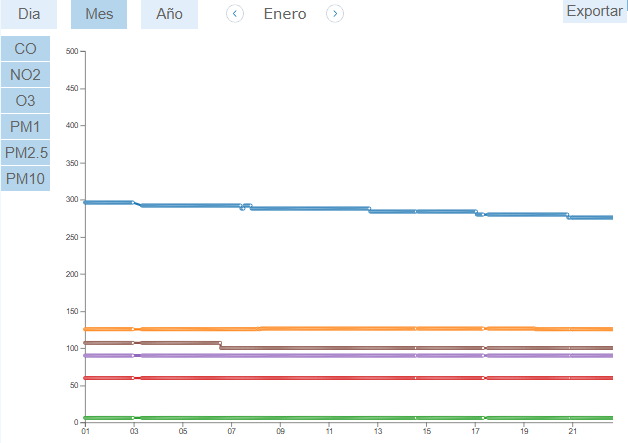
\includegraphics[width=5.75cm]{Figure_4_4_3_a_lineChart}}
        \hfill
    \subfigure [AQI components]
        {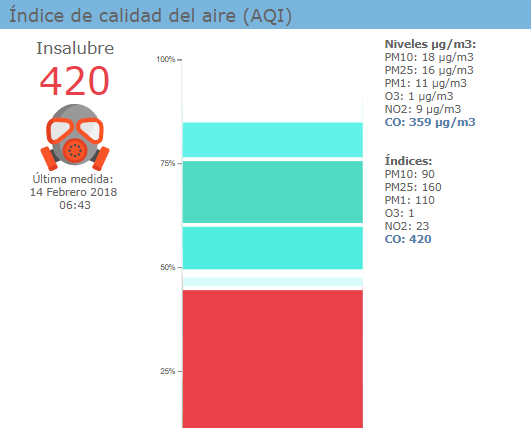
\includegraphics[width=5.25cm]{Figure_4_4_3_b_stakedBarChart}}
    \caption{Charts}
\end{figure}

\begin{center}
    \bf{ (a) AQI Evolution     (b) AQI components   \\
    Figure 4.4.3. Charts}
\end{center}
In addition, to explain the concept of AQI and create an awareness about the influence of air pollution, Aire Guru includes it in the
glossary. This aids understanding of why air pollution should matter to us, with descriptions of the pollutants, medical complications, sources of contamination, the iconography used and
an explanation of what AQI is and how it is calculated. \\